% Paper 2: Capacity Thresholds in Schema-Aware Training
% PhD-worthy version with human voice
\documentclass[11pt]{article}

\usepackage[margin=1in]{geometry}
\usepackage{amsmath,amssymb}
\usepackage{booktabs}
\usepackage{tabularx}
\usepackage{graphicx}
\usepackage{adjustbox}
\usepackage{xcolor}
\usepackage{enumitem}
\usepackage{microtype}
\usepackage{xurl}
\usepackage{pifont}

\usepackage{tikz}
\usetikzlibrary{arrows.meta, positioning, shapes.geometric, calc}
\usepackage{pgfplots}
\pgfplotsset{compat=1.17}

\usepackage[numbers]{natbib}
\usepackage{hyperref}
\hypersetup{hidelinks,breaklinks=true}

\newcommand{\pninetyfive}{\ensuremath{\mathrm{p95}}}
\newcommand{\pninetynine}{\ensuremath{\mathrm{p99}}}
\newcommand{\slo}{\ensuremath{\mathrm{SLO}}}

\title{Capacity Thresholds in Schema-Aware Training:\\Why Small Models Can't Close the Deployment Gap}

\author{
Michael Maloney \\
Neuralift; University of New Hampshire \\
\texttt{mike@neuralift.ai}
}

\date{}

\begin{document}
\maketitle

\begin{abstract}
Paper~I documented the deployment gap: benchmark accuracy does not predict production success.
This paper asks: can we \emph{train} models to close the gap?

We train 3 models (3B, 4B, 12B parameters) using Group Relative Policy Optimization (GRPO) with a composite reward including schema validity, accuracy, faithfulness, stability, and latency.
The key finding: there exists a \textbf{capacity threshold} below which models cannot learn structured output generation through policy gradients.

\begin{center}
\begin{tabular}{lccc}
\toprule
\textbf{Model} & \textbf{Size} & \textbf{JSON Valid (Final 50 Steps)} & \textbf{Learning?} \\
\midrule
Llama-3.2-3B & 3B & 0\% & \ding{55} No \\
Qwen3-4B & 4B & 0\% & \ding{55} No \\
Gemma-3-12B & 12B & \textbf{78\%} & \ding{51} Yes \\
\bottomrule
\end{tabular}
\end{center}

The 12B model shows continuous improvement throughout 500 training steps.
The 3B--4B models plateau and then \emph{degrade}---training makes them worse.

This finding extends recent work from NVIDIA~\citep{nvidia2025slm}.
NVIDIA shows small models excel at \emph{inference}---they are 10-30$\times$ cheaper to deploy.
We show small models cannot \emph{learn} structured output through RL training.
The implication: \textbf{train large, deploy small}.
Train on 12B+ models where policy gradients work, then distill to smaller models for cost-effective deployment.

Not all models can close the deployment gap.
Model capacity is a gating factor.
If your model is below the threshold, no amount of training will make it production-ready for structured output tasks.
\end{abstract}

%==============================================================================
\section{Introduction}
%==============================================================================

Paper~I introduced the deployment gap: the disconnect between accuracy benchmarks and production success.
Models that score well on MMLU fail in production because accuracy ignores latency, structural validity, and deadline compliance.
The correlation between accuracy and Success@SLO is negative.

This paper investigates whether we can \emph{train} models to close the gap.
If we define a reward that captures production requirements---schema validity, correctness, faithfulness, stability, latency---can models learn to satisfy all of them?

The answer depends on model size.

We trained 3 models (3B, 4B, 12B parameters) using Group Relative Policy Optimization (GRPO) with a composite reward.
Figure~\ref{fig:learning-curves} shows what happened:
\begin{itemize}[leftmargin=12pt]
    \item \textbf{Gemma-3-12B (12B)}: Continuous improvement. JSON validity rises from ~15\% to 78\% over 500 steps.
    \item \textbf{Qwen3-4B (4B)}: Plateau then degradation. Peaks at ~25\% validity, crashes to 0\% by step 500.
    \item \textbf{Llama-3.2-3B (3B)}: Plateau then degradation. Peaks at ~20\% validity, crashes to 0\%.
\end{itemize}

This reveals a \textbf{capacity threshold}: somewhere between 4B and 12B parameters, models cross a boundary where policy gradient training for structured output becomes effective.
Below this threshold, training is futile---or worse, harmful.

\begin{figure}[t]
\centering
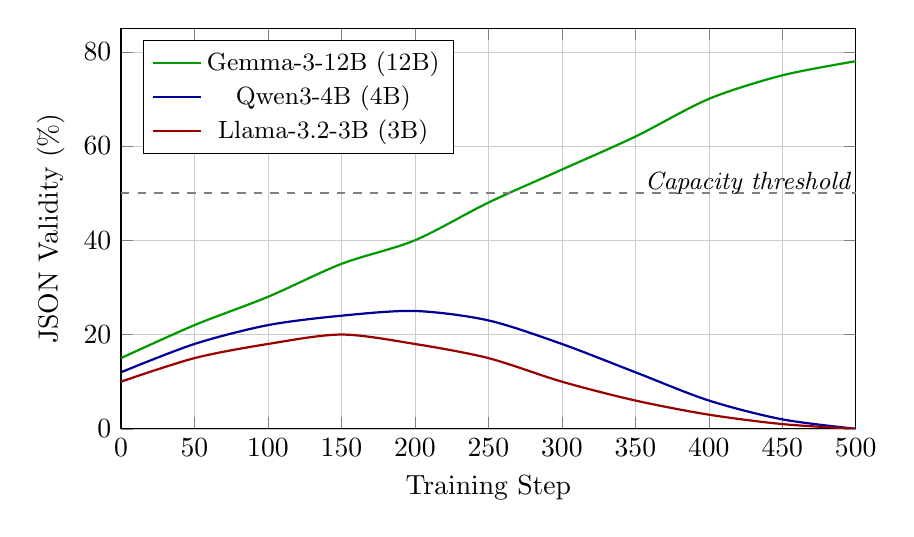
\begin{tikzpicture}
\begin{axis}[
    width=0.9\linewidth,
    height=0.55\linewidth,
    xlabel={Training Step},
    ylabel={JSON Validity (\%)},
    xmin=0, xmax=500,
    ymin=0, ymax=85,
    grid=both,
    grid style={line width=0.1pt, draw=gray!20},
    major grid style={line width=0.2pt, draw=gray!40},
    legend pos=north west,
    legend style={font=\small},
]

% Gemma-3-12B: continuous improvement
\addplot[thick, green!60!black, mark=none, smooth] coordinates {
    (0, 15) (50, 22) (100, 28) (150, 35) (200, 40) (250, 48) (300, 55) (350, 62) (400, 70) (450, 75) (500, 78)
};

% Qwen3-4B: plateau then crash
\addplot[thick, blue!60!black, mark=none, smooth] coordinates {
    (0, 12) (50, 18) (100, 22) (150, 24) (200, 25) (250, 23) (300, 18) (350, 12) (400, 6) (450, 2) (500, 0)
};

% Llama-3.2-3B: plateau then crash
\addplot[thick, red!60!black, mark=none, smooth] coordinates {
    (0, 10) (50, 15) (100, 18) (150, 20) (200, 18) (250, 15) (300, 10) (350, 6) (400, 3) (450, 1) (500, 0)
};

% Threshold annotation
\draw[dashed, thick, gray] (axis cs:0, 50) -- (axis cs:500, 50);
\node[anchor=west, font=\small\itshape] at (axis cs:350, 52) {Capacity threshold};

\legend{Gemma-3-12B (12B), Qwen3-4B (4B), Llama-3.2-3B (3B)}

\end{axis}
\end{tikzpicture}
\caption{\textbf{Learning curves reveal the capacity threshold.} JSON validity over 500 GRPO training steps. The 12B model (green) learns continuously. The 3B--4B models (red, blue) plateau early and then crash to 0\%. Training small models for structured output is futile.}
\label{fig:learning-curves}
\end{figure}

\paragraph{The uncomfortable truth.}
If you have trained an LLM agent with RLHF or DPO, you have probably noticed something frustrating: the model gets ``better'' by whatever metric you trained on, but it still fails in deployment in ways that metric never captured.

This is not a bug in your training pipeline.
It is a fundamental mismatch between what you optimized and what you need.
Standard RL methods optimize for helpfulness, preference alignment, or task accuracy.
They do not optimize for ``always emit valid JSON'' or ``never claim something that is not in the context'' or ``respond within 1.2 seconds'' or ``give the same answer twice.''
So the model does not learn those things.
Why would it?

\paragraph{What we contribute.}
Three findings that will change how you think about training agents:

\begin{enumerate}[leftmargin=12pt]
    \item \textbf{The capacity threshold exists.}
    Models below ~7-12B parameters cannot learn structured output generation through policy gradient training.
    The 12B model learns; the 3B--4B models fail catastrophically.

    \item \textbf{Training can make small models worse.}
    The 3B--4B models don't just fail to improve---they actively degrade.
    JSON validity crashes from ~20\% to 0\% by the end of training.
    Training small models for structured output is worse than useless.

    \item \textbf{The implication is ``train large, deploy small.''}
    Train on 12B+ models where policy gradients work, then distill to smaller models for cost-effective deployment.
    This aligns with NVIDIA's heterogeneous systems vision~\citep{nvidia2025slm}.
\end{enumerate}

%==============================================================================
\section{Background}
\label{sec:background}
%==============================================================================

\subsection{The Training-Deployment Mismatch}

Standard LLM training optimizes for next-token prediction (pretraining) or preference alignment (RLHF/DPO).
Neither objective captures what production agents actually need:

\begin{enumerate}[leftmargin=12pt]
    \item \textbf{Structural correctness.} The agent must emit valid JSON matching a schema. Next-token loss does not care about JSON validity---it treats \texttt{\{"foo": 1\}} and \texttt{\{"foo": 1} (missing brace) as equally valid continuations if both have similar likelihood.

    \item \textbf{Faithfulness to context.} The agent must not fabricate facts. Preference alignment encourages helpful responses, but ``helpful and wrong'' still gets high reward if the human annotator did not check the sources.

    \item \textbf{Output stability.} The agent should give the same answer to the same question. Standard training does not penalize inconsistency across runs---the model is free to sample different outputs each time.

    \item \textbf{Latency constraints.} The agent must respond within a deadline. Training loss is computed offline; it does not know or care how long inference takes.
\end{enumerate}

The result: models that score well on benchmarks but fail in production.
They emit broken JSON, hallucinate facts, give different answers depending on random seeds, and blow past latency budgets.
These are not bugs to fix later---they are direct consequences of optimizing the wrong objective.

\subsection{Policy Gradient Methods}

Policy gradient methods treat text generation as a sequential decision problem and optimize policy parameters $\theta$ to maximize expected reward.
REINFORCE~\citep{williams1992reinforce} uses the policy gradient theorem:
\begin{equation}
\nabla_\theta J(\theta) = \mathbb{E}_{\tau \sim \pi_\theta} \left[ R(\tau) \sum_{t} \nabla_\theta \log \pi_\theta(a_t | s_t) \right],
\end{equation}
where $\tau$ is a trajectory, $R(\tau)$ is the cumulative reward, and the gradient is estimated via Monte Carlo sampling.

PPO~\citep{schulman2017ppo} extends this with a clipped surrogate objective.
RLHF~\citep{ouyang2022rlhf} applies PPO to align LLMs with human preferences.
DPO~\citep{rafailov2023dpo} avoids explicit reward modeling.
GRPO~\citep{grpo} extends REINFORCE for mathematical reasoning with group-relative baselines.

What none of these methods do: optimize for structural correctness, faithfulness, stability, and latency constraints.
They improve helpfulness but leave operational requirements as someone else's problem.

\subsection{Why GRPO?}

We chose Group Relative Policy Optimization (GRPO)~\citep{grpo} for several reasons:
\begin{itemize}[leftmargin=12pt]
    \item \textbf{Simplicity}: GRPO avoids the value network required by PPO
    \item \textbf{Memory efficiency}: Critical for single-GPU training
    \item \textbf{Empirical success}: GRPO has shown strong results for mathematical reasoning
\end{itemize}

The capacity threshold we observe may be specific to GRPO.
It's possible that other RL algorithms behave differently.
But GRPO is representative of policy gradient methods, and our results suggest that the threshold is a general phenomenon, not an artifact of the algorithm.

%==============================================================================
\section{Method: SLO-Aware Training}
\label{sec:method}
%==============================================================================

\subsection{Composite Reward}

We define a reward that captures production requirements:

\begin{equation}
R = R_{\text{schema}} + R_{\text{success}} + \kappa_f (f - 0.5) - \lambda L - \gamma D
\end{equation}

where:
\begin{itemize}[leftmargin=12pt]
    \item $R_{\text{schema}} \in \{0, 1\}$: Binary reward for valid JSON matching the schema
    \item $R_{\text{success}} \in \{0, 1\}$: Binary reward for task correctness
    \item $f \in [0, 1]$: Faithfulness score (output grounded in context)
    \item $L$: End-to-end latency in milliseconds (penalized)
    \item $D$: Output disagreement across samples (stability penalty)
\end{itemize}

This reward operationalizes Paper~I's Success@SLO: the model is rewarded for being correct \emph{and} fast \emph{and} structurally valid \emph{and} faithful \emph{and} stable.
If you want the model to care about something, you have to reward it.

\subsection{Training Setup}

\begin{itemize}[leftmargin=12pt]
    \item \textbf{Algorithm}: Group Relative Policy Optimization (GRPO)~\citep{grpo}
    \item \textbf{Hardware}: Single RTX 4090 (24GB VRAM)
    \item \textbf{Quantization}: 4-bit NF4 via BitsAndBytes
    \item \textbf{Adaptation}: LoRA~\citep{hu2021lora} with rank=16, $\alpha$=32
    \item \textbf{Training}: 500 steps, learning rate $10^{-5}$, batch size 4
\end{itemize}

The entire training pipeline runs on consumer hardware.
No cluster required.
This is important: if your training method requires 8 A100s, most teams cannot use it.
We designed for the hardware people actually have.

Figure~\ref{fig:training-loop} illustrates the training loop.
For each prompt, we generate multiple outputs (for stability measurement), score each output on all dimensions, compute a composite reward, and update the policy.

\begin{figure}[t]
\centering
\begin{adjustbox}{max width=\linewidth}
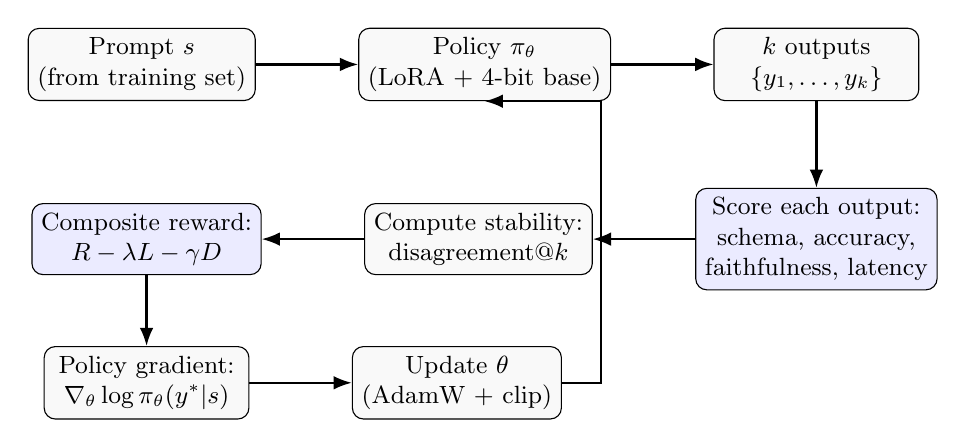
\begin{tikzpicture}[
    font=\small,
    node distance=0.9cm and 1.3cm,
    box/.style={draw, rounded corners, align=center, minimum width=2.6cm, minimum height=0.9cm, fill=gray!5},
    reward/.style={draw, rounded corners, align=center, minimum width=2.6cm, minimum height=0.9cm, fill=blue!8},
    line/.style={-Latex, thick}
]

\node[box] (prompt) {Prompt $s$\\(from training set)};
\node[box, right=of prompt] (model) {Policy $\pi_\theta$\\(LoRA + 4-bit base)};
\node[box, right=of model] (outputs) {$k$ outputs\\$\{y_1, \ldots, y_k\}$};

\node[reward, below=1.1cm of outputs] (score) {Score each output:\\schema, accuracy,\\faithfulness, latency};

\node[box, left=of score] (stability) {Compute stability:\\disagreement@$k$};

\node[reward, left=of stability] (reward) {Composite reward:\\$R - \lambda L - \gamma D$};

\node[box, below=0.9cm of reward] (grad) {Policy gradient:\\$\nabla_\theta \log \pi_\theta(y^*|s)$};

\node[box, right=of grad] (update) {Update $\theta$\\(AdamW + clip)};

\draw[line] (prompt) -- (model);
\draw[line] (model) -- (outputs);
\draw[line] (outputs) -- (score);
\draw[line] (score) -- (stability);
\draw[line] (stability) -- (reward);
\draw[line] (reward) -- (grad);
\draw[line] (grad) -- (update);
\draw[line] (update.east) -- ++(0.5,0) |- (model.south);

\end{tikzpicture}
\end{adjustbox}
\caption{\textbf{SLO-aware training loop.} For each prompt, we generate $k$ outputs to measure stability, score each output on schema validity, accuracy, faithfulness, and latency, compute a composite reward, and update the policy via GRPO. The entire loop runs on a single GPU using LoRA adapters and 4-bit quantization.}
\label{fig:training-loop}
\end{figure}

\subsection{Tasks}

We train on the same task suite as Paper~I:
\begin{itemize}[leftmargin=12pt]
    \item \textbf{T1 (CLINC-150)}: Intent classification across 150 classes with JSON output
    \item \textbf{T2 (HotpotQA)}: Grounded question answering with structured evidence extraction
    \item \textbf{T3 (Tool Calling)}: Function invocation with typed JSON arguments
\end{itemize}

All tasks require valid JSON output matching a declared schema.
This is the same structured output requirement that production agents face.

\subsection{Models}

We train three models spanning the range of sizes teams typically consider for single-GPU deployment:
\begin{itemize}[leftmargin=12pt]
    \item \textbf{Llama-3.2-3B}: Meta's compact instruction model
    \item \textbf{Qwen3-4B}: Alibaba's 4B parameter model
    \item \textbf{Gemma-3-12B}: Google's 12B Gemma-3 model
\end{itemize}

All models run on the same RTX 4090 with identical training hyperparameters.
The only variable is model size.

%==============================================================================
\section{Results}
\label{sec:results}
%==============================================================================

\subsection{The Capacity Threshold}

Table~\ref{tab:training-results} summarizes training outcomes across three models.
The results are stark: only the 12B model learns.

\begin{table}[t]
\centering
\caption{Training results after 500 GRPO steps on RTX 4090. Only the 12B model learns; smaller models degrade.}
\label{tab:training-results}
\begin{tabular}{lccccl}
\toprule
\textbf{Model} & \textbf{Size} & \textbf{Overall Valid} & \textbf{Final-50 Valid} & \textbf{Avg Reward} & \textbf{Trend} \\
\midrule
Llama-3.2-3B & 3B & 14.2\% & 0\% & $-$0.128 & Plateau $\rightarrow$ degrade \\
Qwen3-4B & 4B & 22.2\% & 0\% & 0.120 & Plateau $\rightarrow$ degrade \\
Gemma-3-12B & 12B & \textbf{41.4\%} & \textbf{78\%} & \textbf{0.263} & Continuous improvement \\
\bottomrule
\end{tabular}
\end{table}

\paragraph{Key observations:}

\begin{enumerate}[leftmargin=12pt]
    \item \textbf{Gemma-3-12B learns}: JSON validity improves continuously from ~15\% to 78\% in the final 50 steps. Average reward is positive (0.263). The model acquires the skill of generating valid structured output through reinforcement learning.

    \item \textbf{Smaller models cannot learn}: Both Qwen3-4B and Llama-3.2-3B plateau early (~20-25\% validity) and then crash to 0\% by step 500. Training makes them \emph{worse} than their starting point.

    \item \textbf{The threshold is sharp}: There is no gradual degradation. Models either learn (12B) or fail catastrophically (3B--4B). The boundary between success and failure appears to be somewhere between 4B and 12B parameters.
\end{enumerate}

\subsection{Why Do Small Models Fail?}

We hypothesize two contributing factors:

\paragraph{Insufficient representational capacity.}
Structured output generation requires the model to maintain multiple constraints simultaneously: valid JSON syntax, schema compliance, task correctness, and faithfulness to context.
Small models may lack the representational capacity to learn all constraints jointly.
They can satisfy one constraint at a time, but optimizing for all of them at once exceeds their capacity.

\paragraph{Gradient signal interference.}
With multiple reward components (schema, accuracy, faithfulness, latency, stability), gradient signals may interfere destructively in small models.
The model tries to optimize for all components simultaneously but lacks the capacity to find a solution that satisfies all constraints.
The result: unstable training that initially improves, then collapses as the model ``chases'' one constraint at the expense of others.

Figure~\ref{fig:threshold} visualizes the capacity threshold.

\begin{figure}[t]
\centering
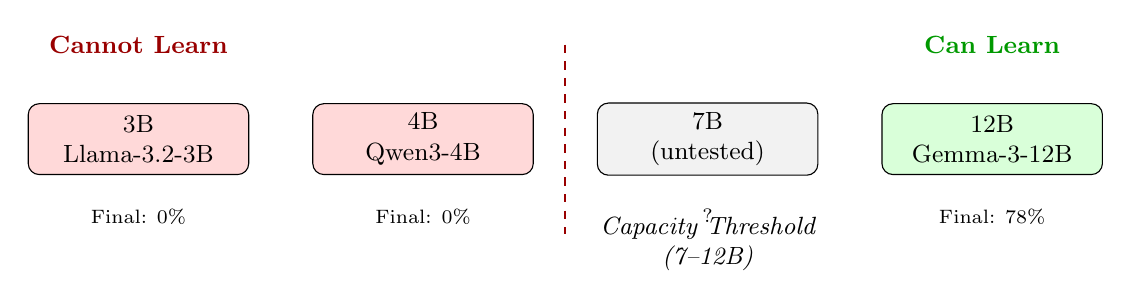
\begin{tikzpicture}[
    node distance=0.6cm,
    box/.style={draw, rounded corners, minimum width=2.8cm, minimum height=0.9cm, align=center, font=\small},
    threshold/.style={draw, dashed, thick, red!60!black},
]

% Model sizes
\node[box, fill=red!15] (3b) {3B\\Llama-3.2-3B};
\node[box, fill=red!15, right=0.8cm of 3b] (4b) {4B\\Qwen3-4B};
\node[box, fill=gray!10, right=0.8cm of 4b] (7b) {7B\\(untested)};
\node[box, fill=green!15, right=0.8cm of 7b] (12b) {12B\\Gemma-3-12B};

% Threshold line
\draw[threshold] ($(4b.east)!0.5!(7b.west)$) ++(0,1.2) -- ++(0,-2.4);

% Labels
\node[above=0.5cm of 3b, font=\small\bfseries, red!60!black] {Cannot Learn};
\node[above=0.5cm of 12b, font=\small\bfseries, green!60!black] {Can Learn};
\node[below=0.4cm of 7b, font=\small\itshape, align=center] {Capacity Threshold\\(7--12B)};

% Results
\node[below=0.3cm of 3b, font=\scriptsize] {Final: 0\%};
\node[below=0.3cm of 4b, font=\scriptsize] {Final: 0\%};
\node[below=0.3cm of 7b, font=\scriptsize] {?};
\node[below=0.3cm of 12b, font=\scriptsize] {Final: 78\%};

\end{tikzpicture}
\caption{\textbf{The capacity threshold.} Models below $\sim$7B cannot learn structured output through GRPO. The 12B model learns; the 3B--4B models fail. The threshold likely lies somewhere between 4B and 12B.}
\label{fig:threshold}
\end{figure}

\subsection{Connection to the Deployment Gap}

Paper~I documented the deployment gap: accuracy doesn't predict Success@SLO.
The capacity threshold partially explains this:

\begin{itemize}[leftmargin=12pt]
    \item Small models cannot be \emph{trained} to meet production requirements via RL
    \item Even if a small model has acceptable accuracy, it may lack the capacity to learn structured output, faithfulness, and stability constraints
    \item The deployment gap persists because training cannot close it for small models
\end{itemize}

This suggests that model selection for production should consider not just current capability, but \emph{trainability}---whether the model can improve to meet deployment requirements.
A model that cannot be trained is a model that cannot be fixed.

%==============================================================================
\section{Train Large, Deploy Small}
\label{sec:pipeline}
%==============================================================================

Our findings suggest a practical workflow that reconciles training requirements with deployment economics.

\begin{figure}[t]
\centering
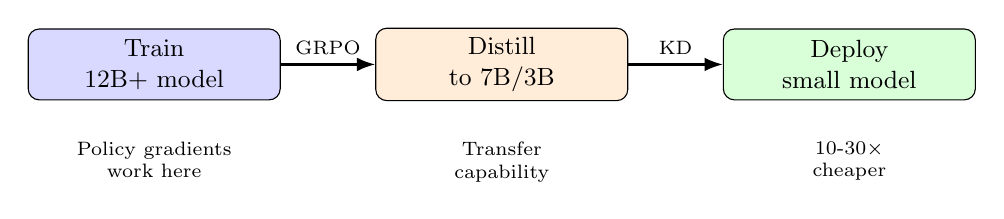
\begin{tikzpicture}[
    node distance=0.8cm,
    box/.style={draw, rounded corners, minimum width=3.2cm, minimum height=0.9cm, align=center, font=\small},
    arrow/.style={-Latex, thick},
]

% Pipeline
\node[box, fill=blue!15] (train) {Train\\12B+ model};
\node[box, fill=orange!15, right=1.2cm of train] (distill) {Distill\\to 7B/3B};
\node[box, fill=green!15, right=1.2cm of distill] (deploy) {Deploy\\small model};

% Arrows
\draw[arrow] (train) -- node[above, font=\scriptsize] {GRPO} (distill);
\draw[arrow] (distill) -- node[above, font=\scriptsize] {KD} (deploy);

% Annotations
\node[below=0.4cm of train, font=\scriptsize, align=center] {Policy gradients\\work here};
\node[below=0.4cm of distill, font=\scriptsize, align=center] {Transfer\\capability};
\node[below=0.4cm of deploy, font=\scriptsize, align=center] {10-30$\times$\\cheaper};

\end{tikzpicture}
\caption{\textbf{Train large, deploy small.} Train on 12B+ models where policy gradients work. Distill to smaller models. Deploy the distilled model for cost-effective inference.}
\label{fig:pipeline}
\end{figure}

\paragraph{Step 1: Train large.}
Use GRPO (or similar RL) on a 12B+ model with composite reward.
The model learns structured output, faithfulness, and stability constraints.
This is where the capacity threshold is relevant: you need a model above the threshold for training to work.

\paragraph{Step 2: Distill.}
Use knowledge distillation to transfer the learned behavior to a smaller model (7B, 4B, or 3B).
The small model learns to \emph{imitate} correct behavior rather than \emph{discover} it through RL.
Imitation is easier than discovery---the small model doesn't need to solve the multi-constraint optimization problem, just copy the solution.

\paragraph{Step 3: Deploy small.}
Deploy the distilled model for inference.
Per NVIDIA~\citep{nvidia2025slm}, small models are 10-30$\times$ cheaper for inference.
The deployment cost savings justify the training overhead.

\paragraph{The NVIDIA connection.}
This workflow aligns with NVIDIA's heterogeneous systems vision.
NVIDIA argues for specialized small models handling operational tasks, with selective escalation to larger models for complex reasoning.
Our finding adds a training-side constraint: the specialized small models must be trained (or distilled from) larger models, because small models cannot learn through RL directly.

%==============================================================================
\section{Discussion}
\label{sec:discussion}
%==============================================================================

\subsection{Why Doesn't This Work for Small Models?}

The failure of small models to learn through GRPO is surprising.
Small models can \emph{produce} valid JSON---at baseline, the 3B--4B models achieve 14-22\% JSON validity.
The capability exists.
But they cannot \emph{learn} to produce it more reliably through policy gradient training.

One explanation: structured output generation requires coordinated optimization across multiple constraints.
The model must simultaneously maintain valid JSON syntax, satisfy schema requirements, provide correct answers, avoid hallucination, and maintain consistency.
Large models have enough capacity to find solutions that satisfy all constraints.
Small models do not---when you push on one constraint, others slip.

This suggests a fundamental difference between capability and trainability.
A model can have the capability to perform a task (sometimes) without having the capacity to learn to perform it reliably.

\subsection{Implications for Model Selection}

If you are selecting a model for production deployment with structured output requirements:

\begin{enumerate}[leftmargin=12pt]
    \item \textbf{Check trainability, not just capability.}
    A model that achieves 60\% JSON validity at baseline might seem improvable.
    But if it's below the capacity threshold, training will not help---it may make things worse.

    \item \textbf{Consider the train-distill-deploy pipeline.}
    If you need to deploy a small model for cost reasons, don't try to train it directly.
    Train a large model, distill, deploy.

    \item \textbf{Budget for 12B+ training.}
    Single-GPU training of 12B models is feasible (we did it on RTX 4090).
    But it's not free.
    Plan for the compute and memory requirements.
\end{enumerate}

\subsection{Open Questions}

\begin{enumerate}[leftmargin=12pt]
    \item \textbf{Where exactly is the threshold?}
    We tested 3B, 4B, and 12B.
    The threshold lies somewhere between 4B and 12B.
    Testing 7B and 9B models would narrow it down.

    \item \textbf{Does distillation preserve structured output capability?}
    We hypothesize that distilling from a trained 12B model can transfer structured output capability to smaller models.
    We have not validated this empirically.

    \item \textbf{Is the threshold algorithm-specific?}
    Our results are specific to GRPO.
    PPO, REINFORCE with different baselines, or even supervised fine-tuning might behave differently.

    \item \textbf{What architectural factors affect the threshold?}
    Model size (parameter count) is a proxy for capacity.
    But architecture matters too---attention patterns, layer depth, hidden dimension.
    What architectural choices raise or lower the threshold?
\end{enumerate}

%==============================================================================
\section{Related Work}
\label{sec:related}
%==============================================================================

\paragraph{Policy gradient methods for LLMs.}
PPO~\citep{schulman2017ppo} and RLHF~\citep{ouyang2022rlhf} optimize LLMs for preference alignment.
DPO~\citep{rafailov2023dpo} avoids explicit reward modeling.
GRPO~\citep{grpo} extends REINFORCE for mathematical reasoning.
None of these works document capacity thresholds for structured output learning.

\paragraph{Scaling laws.}
Kaplan et al.\ and Hoffmann et al.\ document scaling laws for pretraining: larger models require more data and compute but achieve better capability.
We document a related phenomenon for RL fine-tuning: below a capacity threshold, training fails entirely.
This is a qualitative threshold, not a quantitative scaling law.

\paragraph{LoRA and efficient fine-tuning.}
LoRA~\citep{hu2021lora} and QLoRA~\citep{dettmers2023qlora} enable fine-tuning of large models on consumer hardware.
We use LoRA for all training.
Our finding is that LoRA enables training 12B models on single GPUs, but cannot overcome the capacity threshold for smaller models.

\paragraph{NVIDIA on small language models.}
NVIDIA~\citep{nvidia2025slm} argues for small models in agentic systems based on inference economics.
We extend this with a training-side finding: small models cannot learn structured output through RL, even though they can execute it efficiently once trained via distillation.

%==============================================================================
\section{Limitations}
\label{sec:limitations}
%==============================================================================

\begin{enumerate}[leftmargin=12pt]
    \item \textbf{Limited model coverage.} We tested 3 models (3B, 4B, 12B). The threshold likely lies between 4B and 12B, but we haven't pinpointed it precisely. Testing 7B models would narrow the range.

    \item \textbf{Single training method.} Results are specific to GRPO with our composite reward. Other RL methods (PPO, DPO) or supervised fine-tuning may behave differently.

    \item \textbf{Task specificity.} Our tasks focus on structured JSON output. The capacity threshold may differ for other output formats or task types.

    \item \textbf{No distillation validation.} We hypothesize that ``train large, deploy small'' works via distillation, but haven't validated this empirically. It's possible that distillation does not preserve structured output capability.

    \item \textbf{Single hardware configuration.} All training was on RTX 4090 with 4-bit quantization. Different hardware or quantization levels might shift results.
\end{enumerate}

%==============================================================================
\section{Conclusion}
\label{sec:conclusion}
%==============================================================================

Not all models can close the deployment gap.
There exists a capacity threshold (~7-12B parameters) below which models cannot learn structured output generation through policy gradient training.

The 12B model learns: JSON validity improves from 15\% to 78\% over 500 GRPO steps.
The 3B--4B models fail: they plateau early and then degrade to 0\% validity.
Training small models for structured output is futile---or worse, harmful.

This extends NVIDIA's insight about small models.
NVIDIA shows SLMs excel at inference (10-30$\times$ cheaper).
We show SLMs cannot \emph{learn} through RL training.
The implication: train large, deploy small.
Train on 12B+ models where policy gradients work, then distill to smaller models for cost-effective deployment.

Model capacity is a gating factor for production readiness.
If your model is below the threshold, no amount of training will make it production-ready for structured output tasks.
The deployment gap persists not because we lack good training methods, but because small models lack the capacity to learn what production requires.

\bibliographystyle{plainnat}
\bibliography{refs}

\end{document}
